Probabilistic Seismic Hazard, a methodology largely 
founded on the works of \citet{cornell1968} and \citet{esteva1968}, 
nowadays contains a well established system of methods. 
%
The development of PSHA within the latest four decades did not change much of 
the original concept but made calculations more rigorous and accurate, 
especially with respect to the treatment of uncertainties. 

The evolution of PSHA methodologies proceeded in parallel with the development 
of instrumental seismology and hardware computing power. Computer codes such as
EQRISK \citep{mcguire1976} and the sequential versions of SEISRISK
\citep{bender1982,bender1987} traced the advancement of PSHA calculation within
the last part of the 20th century.

At the present time, the most computationally intensive PSHA models available 
are the ones developed for site-specific PSHA analyses, such as the ones 
performed for special installations or advanced regional PSHA input models 
(e.g. the UCERF2 model, \citet{field2009}) and the one used for large areas 
(e.g. continents or large nations) require powerful calculation facilities 
and sophisticated codes.
%
The computation demand posed by these model derives in the first case from 
the complexity of the input whilst in the second case is the number of sites 
that renders calculations particularly heavy.  

OpenQuake tries to cover this growing requirement for an accessible and 
efficient code for PSHA calculation. It's worth noting that the hazard 
component of OpenQuake leverages from OpenSHA (http://www.opensha.org) - 
an advanced, open-source, Java-based platform for conducting Seismic 
Hazard Analysis - and it is currently developed in collaboration with 
the OpenSHA team.  
%
% ------------------------------------------------------------------------------
\section{OpenQuake-hazard: main concepts}
Schematically, the procedure that OpenQuake follows to compute probabilistic 
seismic hazard is the following:
%
\begin{enumerate}
%
\item \emph{Read the PSHA input model - i.e. the union of the Seismic Sources 
System and the Ground Motion Model System - and calculation 
settings.}
	\index{Seismic Sources!System} %%%%%%
	\index{PSHA!Input model} %%%%%%
	\index{Ground Motion!System} %%%%%%
	
	The \emph{Seismic Sources System} is an object that contains the 
	information necessary to create one or several Seismic Sources Model, 
	eventually by taking into account the epistemic uncertainties. 
	%
	The Seismic Sources System contains:
	\begin{itemize}
	\item One or several \emph{Initial Seismic Sources Models};
	\index{Logic Tree!Seismic Sources} %%%%%%
	\item One logic tree - the Seismic Sources Logic Tree - describing 
	epistemic uncertainties connected with the objects and parameters 
	characterizing the Initial Seismic Sources Models.
	\end{itemize}
	
	The Ground Motion System is an object that contains the information 
	necessary to create (or use) one or several Ground Motion models, eventually 
	by taking into account the epistemic uncertainties. 
	\begin{itemize}
	\item One or several Ground Motion Models;
	\index{Logic Tree!Ground Motion} %%%%%%
	\item One logic tree - the Ground Motion Model Logic Tree - 
	describing epistemic uncertainties connected with the objects and 
	parameters characterizing the selected Ground Motion Models.	
	\end{itemize}

%
\item \emph{Process the logic tree structures to account for epistemic 
uncertainties connected with the seismic sources and ground motion, 
create Seismic Sources Models and Ground Motion Models}.
	\index{Seismic Sources!Model} %%%%%%
	\index{Ground Motion!Model} %%%%%%
	
	A Seismic Sources Model contains the information necessary to create an 
	Earthquake Rupture Forecast (i.e. the probabilistic seismicity occurrence
	model) without con\-sid\-er\-ing any epistemic uncertainty.
	%
	A Ground Motion Prediction E\-qua\-tions Model includes the information 
	necessary to compute hazard using a Seismic Sources Model. 
\item \emph{Compute the hazard considering as many Seismic Sources Models and 
Ground Motion Prediction Equations Models as need to adequately characterize 
uncertainties}.
\item \emph{Post-process the results obtained for distinct calculations}.
\end{enumerate}
%
% ------------------------------------------------------------------------------
\section{Calculation workflows}
% Three types of analysis
The hazard component of OpenQuake-Hazard performs seismic hazard 
analysis (SHA) following various approaches. 
%
Currently three main types of analysis are supported:
\begin{itemize}
\item \textit{Classical Probabilistic Seismic Hazard Analysis (cPSHA)}, 
allowing calculation of hazard curves and hazard maps following 
classical integration procedure 
(\cite{cornell1968}) as formulated by \cite{field2003}).
\item \textit{Event-Based Probabilistic Seismic Hazard Analysis (ePSHA)}, 
allowing calculation of ground motion fields from stochastic event sets.
\item \textit{Deterministic SHA (DSHA)}, allowing calculation of ground motion 
fields from single earthquake rupture scenario.
\end{itemize}
Each type of analysis has a modular structure, thus providing the capability 
of investigating all possible intermediate results. Moreover, each calculator 
can be expanded independently so that more calculation options/methodologies 
can be easily introduced, without affecting the overall calculation workflow.

Indeed each workflow described in the following Sections involves a number 
of calculators, each responsible for a specific task. 
Figures \ref{classical_psha_workflow}, \ref{event_based_workflow}, and 
\ref{deterministic_workflow} schematically depict the different calculation 
workflows.
%
%  - - - - - - - - - - - - - - - - - - - - - - - - - - - - - - - - - - - - - - -
\subsection{Classical Probabilistic Seismic Hazard Analysis}
\label{section:classicalPSHA}
%
Input data for the classical PSHA consist of a PSHA Input Model (PSHAim) that 
is provided together with a set of calculation settings. 
%
Chapter \ref{chap:hazinp} describes extensively the content of a PSHAim and 
in particular the different options for modeling seismogenic sources and the 
option offered to include epistemic uncertainties on both seismicity and 
ground motion models in the form of a logic tree; Chapter \ref{chap:hazinp} 
also incorporates the description of the logic tree structure adopted.
%
% ..............................................................................
% . . . . . . . . . . . . . . . . . . . . . . . . . . . . . . . . . . . > Figure
\begin{figure}[htbp]
\begin{center}
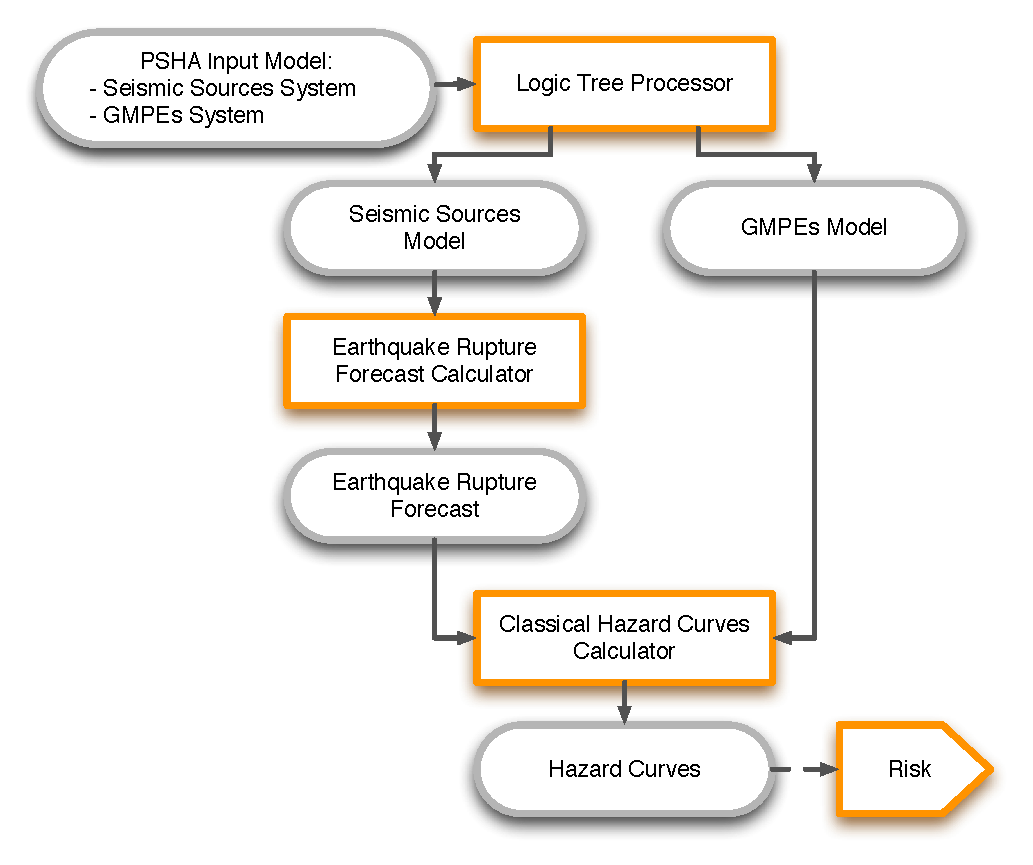
\includegraphics[width=12cm]{./Figures/Part_Hazard/classical_psha_workflow.eps}
\caption{Workflow for classical PSHA (boxes with purple border represent the 
calculators). Given a PSHA Input Model 
the Logic Tree Processor is responsible for creating a Seismic Sources model
and a ground motion model. 
The Seismic Sources model is then provided to the Earthquake Rupture Forecast 
calculator, which computes the ERF (the list of all earthquake ruptures in the 
source model with their probabilities of occurrence). 
Using the ERF and the GMPEs model the Classical PSHA calculator produces 
curves at the sites of interest.}
\label{classical_psha_workflow}
\end{center}
\end{figure}
% . . . . . . . . . . . . . . . . . . . . . . . . . . . . . . . . . . . < Figure
% ..............................................................................

As represented in Figure \ref{classical_psha_workflow}, the main calculators 
used to perform this analysis are:
\begin{enumerate}
%
\item \emph{Logic Tree Processor} \hfill \\
The Logic Tree Processor takes as an input the PSHA Input model. In case of 
the Seismic Sources, using the one of the Initial Seismic Sources Models and 
and by 'harvesting' the information contained in the Seismic Sources Logic Tree
- that is to sample the epistemic uncertainties - it creates a Seismic Sources 
Model (i.e. a model describing geometry and activity rates of each source 
without any epistemic uncertainty). 
%
Following the procedure just described the Logic Tree Processor creates a 
Ground Motion model (i.e. a data structure that associates to each tectonic 
region considered in the calculation a GMPE).
%
\item \emph{Earthquake Rupture Forecast Calculator} \hfill \\
The produced Seismic Sources Model is then used as input for the Earthquake 
Rupture Forecast (ERF) calculator which computes the probability of occurrence, 
over a specified time span, for each earthquake rupture produced by the source 
model.
\item \emph{Classical PSHA Calculator} \hfill \\
The cPSHA uses the ERF and the Ground Motion model to compute hazard curves on 
each site specified in the calculation settings.
\end{enumerate} 
%
%  - - - - - - - - - - - - - - - - - - - - - - - - - - - - - - - - - - - - - - -
\subsection{Event-Based Probabilistic Seismic Hazard Analysis}
\label{section:event-basedPSHA}
Input data for the Event-Based PSHA - as in the case of the Classical PSHA 
calculator - consist of a PSHA Input Model supplied to OQ together with a 
set of calculation settings.
%
% ..............................................................................
% . . . . . . . . . . . . . . . . . . . . . . . . . . . . . . . . . . . > Figure
\begin{figure}
\centering
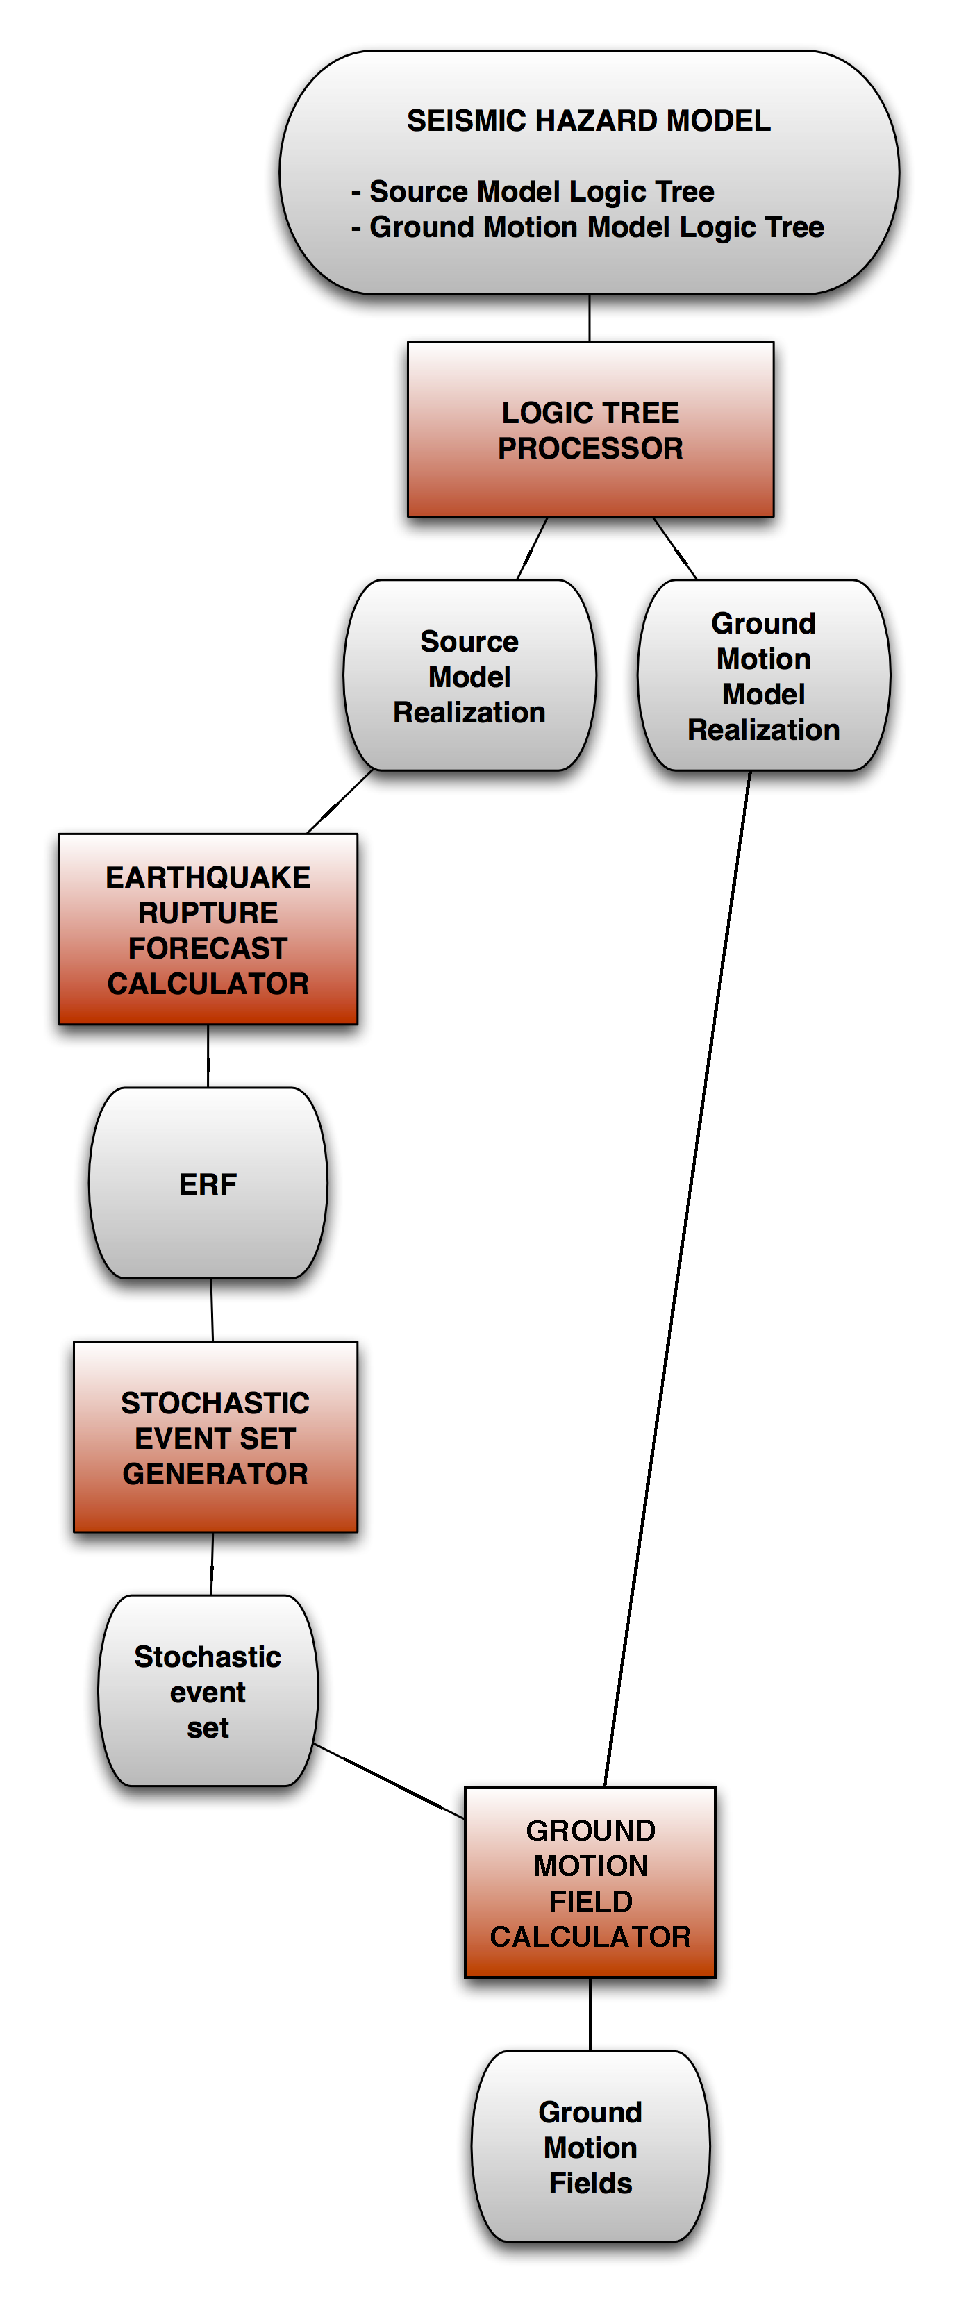
\includegraphics[width=12cm]{./Figures/Part_Hazard/event_based_workflow.eps}
\caption{Workflow for event-based PSHA. Similarly to the classical PSHA workflow 
(Figure \ref{classical_psha_workflow}), an ERF is computed, which is then used 
to generate a stochastic event set (representative of the seismic activity of 
a region in a given time span). Each event is then utilized to calculate a 
ground motion field over a region of interest.}
\label{event_based_workflow}
\end{figure}
% . . . . . . . . . . . . . . . . . . . . . . . . . . . . . . . . . . . < Figure
% ..............................................................................
As represented in Figure \ref{event_based_workflow}, the main calculators 
used to perform this analysis are:
\begin{enumerate}
%
\item \emph{Logic Tree Processor} \hfill \\
The Logic Tree Processor was already 
introduced in the description of the cPSHA workflow (see section 
\ref{section:classicalPSHA} at page \pageref{section:classicalPSHA}).
%
\item \emph{Earthquake Rupture Forecast Calculator} \hfill \\ 
The Logic Tree Processor was already 
introduced in the description of the cPSHA workflow (see section 
\ref{section:classicalPSHA} at page \pageref{section:classicalPSHA}).
%
\item \emph{Stochastic Event Set Calculator} \hfill \\
The Stochastic Event Set Calculator generates a Stochastic Event set 
by sampling each rupture contained in the ERF according to its 
probability of occurrence. Usually a Stochastic Event Set (SES) contains
a large number of seismicity history each one representative of a  
possible collection of events that can be produced by the seismic sources
considered in an analysis during the time span fixed for the calculation
of hazard (normally corresponding to 50 years).
%
\item \emph{Ground Motion Field Calculator} \hfill \\
The Ground Motion Field Calculator computes for each event contained in a 
Stochastic Event Set - provided as an input - a realization of the 
ground shaking taking into account the aleatory uncertainties in 
the ground motion model. Eventually, the Ground Motion Field calculator 
can consider the spatial correlation of the ground motion during the 
generation of the GMF.
%
\item \emph{Event-based PSHA Calculator} \hfill \\
The event-based PSHA calculator takes a (large) set of ground motion 
fields representative of the possible shaking that the investigated 
area can eventually experience over a (large) time span and for each 
grid node in a ground motion fields computes the corresponding hazard 
curve. 
%
This procedure is computationally intensive and is not recommended for 
investigating the hazard over large areas. 
\end{enumerate}

The Logic Tree Processor and the Earthquake rupture forecast were already 
introduced during the descrption of the cPSHA workflow (see section 
\ref{section:classicalPSHA} at page \pageref{section:classicalPSHA}).
%
%  - - - - - - - - - - - - - - - - - - - - - - - - - - - - - - - - - - - - - - -
\subsection{Deterministic Seismic Hazard Analysis}
\label{section:deterministicSHA}
% Deterministic
For deterministic SHA (DSHA), the input data consist of a single earthquake 
rupture model and a single ground motion model. Using the Ground Motion Field 
Calculator, multiple realizations of ground shaking can be computed, each 
realization sampling the aleatory uncertainties in the ground motion model.

As represented in Figure \ref{deterministic_workflow}, the main calculators 
used to perform this analysis are:
\begin{enumerate}
\item \emph{Ground Motion Field Calculator} \hfill \\
The Ground Motion Field Calculator was already 
introduced during the descrption of the ePSHA workflow (see section 
\ref{section:event-basedPSHA} at page \pageref{section:classicalPSHA}).
\end{enumerate}
% ..............................................................................
% . . . . . . . . . . . . . . . . . . . . . . . . . . . . . . . . . . . > Figure
\begin{figure}[!hb]
\centering
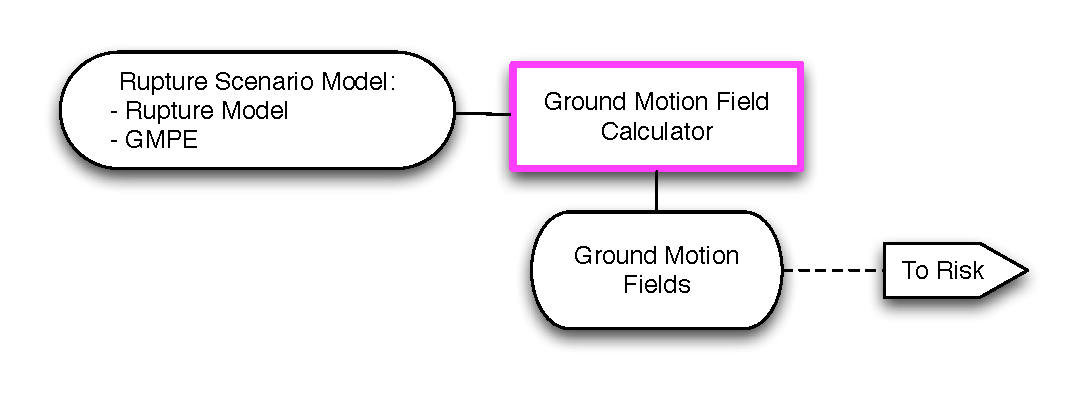
\includegraphics[width=12cm]{./Figures/Part_Hazard/deterministic_workflow.eps}
\caption{Workflow for deterministic SHA. Given a rupture scenario model, 
consisting of an earthquake rupture model, plus a GMPE, the ground motion 
field calculator can compute multiple ground motion field realizations (by 
taking into account GMPE aleatory uncertainties).}
\label{deterministic_workflow}
\end{figure}
% ..............................................................................
% . . . . . . . . . . . . . . . . . . . . . . . . . . . . . . . . . . . > Figure
%
% More details in the next chapters
%Next chapters discuss in more details the data model and the calculators. 
%Chapter \ref{chap:hazinp} describe the input data definition, that is the 
%different options for modeling seismogenic sources and how to include 
%epistemic uncertainties in both seismicity and ground motion models in 
%the form of a logic tree; Chapter \ref{chap:hazinp} also incorporates 
%the description of the logic tree structure adopted. 
%
%The methodology adopted to process the logic tree structure and the 
%definition and modeling of earthquake ruptures for the different 
%seismogenic source typologies are the topics of Chapter \ref{chap:erf}. 
%
%Chapter \ref{chap:hazcalc} describes the theoretical framework behind the main 
%hazard calculator available in OpenQuake: classical PSHA calculator and event 
%based calculator.